\documentclass[conference]{IEEEtran}
\IEEEoverridecommandlockouts
%% ---------------------------------------------------------------------------
%% Glaukopis: Building a 32B CTI LLM Using Chained Instruction Fine-Tuning
%% IEEE Conference template port — targets 38th IEEE ICTAI 2026
%% (https://ictai.computer.org/2026/)
%%
%% Worth, Cardei, Alam. Compile with pdfLaTeX:
%%   pdflatex glaukopis_ieee
%%   bibtex   glaukopis_ieee
%%   pdflatex glaukopis_ieee
%%   pdflatex glaukopis_ieee
%% ---------------------------------------------------------------------------

\usepackage{cite}
\usepackage{amsmath,amssymb,amsfonts}
\usepackage{algorithmic}
\usepackage{graphicx}
\usepackage{textcomp}
\usepackage{xcolor}
\usepackage{url}
\usepackage{hyperref}
\usepackage{booktabs}
\usepackage{array}

\graphicspath{{figures/}{img/}{Fig/}}

%% --- Technical-identifier macro --------------------------------------------
%% \hfid{...} renders a Hugging Face / Hugging Face-style identifier (model
%% name, dataset path, etc.) in a slightly smaller monospaced font that wraps
%% cleanly at `/`, `-`, and `_` boundaries so that long identifiers do not
%% overflow the column. Implemented via the url package with hyphen and
%% underscore added to the break set.
%% --------------------------------------------------------------------------
\makeatletter
\AtBeginDocument{%
  \urlstyle{tt}%
  \def\UrlBreaks{\do\/\do\-\do\_\do\.\do\:}%
}
\makeatother
\providecommand{\hfid}[1]{{\small\nolinkurl{#1}}}

\def\BibTeX{{\rm B\kern-.05em{\sc i\kern-.025em b}\kern-.08em
    T\kern-.1667em\lower.7ex\hbox{E}\kern-.125emX}}

\begin{document}

\title{Glaukopis: Constructing a 32B CTI LLM Using Chained Instruction Fine-Tuning
\thanks{This research was funded by Athena Security Group, LLC.}
}

\author{%
\IEEEauthorblockN{%
  Peter J. Worth Jr.\textsuperscript{1,3,*},\quad
  Ionut Cardei\textsuperscript{1,3},\quad
  Salman Ahmad\textsuperscript{4},\quad
  Muhammad Mamoon Khan\textsuperscript{4}%
}
\IEEEauthorblockA{%
  \textsuperscript{1}\textit{Dept.\ of Electrical Engineering and Computer Science, Florida Atlantic University}, Boca Raton, FL, USA \\
  \textsuperscript{3}\textit{Athena Security Group, LLC}, USA \quad
  \textsuperscript{4}\textit{RevolveAI} \\[2pt]
  \textsuperscript{*}Corresponding author: \texttt{pworthjr@athenasecuritygrp.com}%
}%
}

\maketitle

\begin{abstract}
Cyber threat intelligence (CTI) workflows in regulated security operations cannot in general rely on frontier proprietary models due to cost, latency, and data-handling constraints, while generic foundation models lack the schema fidelity, applied reasoning, and current-threat awareness those workflows require. This paper introduces \textbf{Glaukopis}, a methodology and working system for producing on-premises 32B-scale CTI expert language models via \textit{chained instruction fine-tuning} (chained IFT): an IFT pipeline in which each Alpaca-format (instruction, input, output) triple is materialized by a typed query against an authoritative knowledge graph---so every row is graph-grounded rather than synthesized---and in which the supervised pass is decomposed into a chain of stages with distinct dataset shards and hyperparameter regimes. Glaukopis has three components: \textbf{Ariadne}, a Neo4j substrate ingesting twelve public CTI sources into ${\sim}280$K nodes and ${\sim}480$K edges; \textbf{Sophia}, a graph-template generator that compiles declarative CTI reasoning patterns into IFT triples consistent with the graph; and a \textbf{four-stage IFT chain} (Core, +TAA, CSE, Recalibrate-32B). The v21 ship checkpoint reaches 66.3 average CTI benchmark score (vs.\ 59.0 for its Qwen-2.5-32B-Instruct base), approaching DeepSeek-V4-Pro (70.4), Gemini-3-Flash-Preview (69.8), and GPT-5.5 (72.9) at approximately two orders of magnitude lower per-evaluation cost.
\end{abstract}

\begin{IEEEkeywords}
instruction fine-tuning, chained IFT, supervised fine-tuning, small language models, cyber threat intelligence, CTI knowledge graphs, Neo4j, MITRE ATT\&CK, AthenaBench
\end{IEEEkeywords}

\section{Introduction}

Large language models (LLMs) are now embedded throughout the cyber security workflow: they summarize threat reports, map indicators to MITRE ATT\&CK, triage vulnerabilities, draft detection rules, and answer analyst questions inside security operations centers (SOCs). Surveys of security LLMs consistently identify the same residual failure modes: hallucinations on schema-bearing fields, shallow pattern matching where multi-hop reasoning is required, and a structural inability to operate on threat information more recent than the base model's pretraining cutoff \cite{levi2024cyberpal,liu2024cyberbench}.

\textbf{The operational dilemma.} The industry response has been an awkward two-way split. Generic foundation models are inexpensive and easy to host but underperform on CTI-specific tasks---schema fidelity (CVE/CWE/ATT\&CK identifiers, CVSS vectors), applied reasoning (root-cause mapping, severity estimation, threat-actor attribution), and current-threat awareness are all weak. Frontier proprietary models close much of the gap, but their cost, latency, and data-handling characteristics are incompatible with most regulated security operations: SOCs supporting healthcare, financial, or government workloads cannot, in general, send raw threat telemetry to a third-party API, and the per-evaluation cost of a frontier model across a realistic CTI workload is prohibitive at analyst-team scale.

\textbf{Chained instruction fine-tuning.} A natural alternative is a small (sub-32B) model post-trained on CTI material from authoritative public sources and deployable on-premises. The approach pursued here, \textit{chained instruction fine-tuning} (chained IFT), refines the standard IFT pipeline \cite{wei2022flan,ouyang2022instructgpt,chung2022flant5} along two axes: (i) on the \emph{data} side, every Alpaca-format triple is materialized by a typed query against an authoritative knowledge graph rather than authored or LLM-synthesized, so each row is grounded in named graph nodes traceable to public-source natural keys; and (ii) on the \emph{training} side, the supervised pass is decomposed into a chain of stages with distinct shards and hyperparameter regimes, so capabilities accumulate compositionally and per-axis regressions are attributable to specific stages. The closest neighbors are IBM's CyberPal.AI and SecKnowledge, which couple expert-curated instruction schemas with chain-of-thought enrichment \cite{levi2024cyberpal,levi2025toward}, and SEvenLLM and CyberBench, which adapt smaller open models through hand-crafted or LLM-synthesized corpora \cite{ji2024sevenllm,liu2024cyberbench}.

\textbf{The Glaukopis system.} Glaukopis is the working instantiation of chained IFT, with three named components: \textbf{Ariadne} (Section~\ref{sec:cti-kg}), a Neo4j substrate ingesting twelve public CTI sources into ${\sim}280$K nodes and ${\sim}480$K edges, refreshed daily; \textbf{Sophia} (Section~\ref{sec:cti-kg}), a graph-template generator that compiles declarative CTI reasoning patterns into Alpaca triples whose outputs are computed directly from Cypher queries; and a \textbf{four-stage IFT chain} (Section~\ref{sec:glaukopis})---Core, +TAA, CSE, Recalibrate-32B---each with its own shard, hyperparameter regime, and capability outcome (Figure~\ref{fig:glaukopis-chained-ift}).

\textbf{Headline result.} The v21 ship checkpoint, \hfid{asg-ai/athena-cti-sft-qwen25-32b-v21-recal-32b}, reaches an average CTI-benchmark score of 66.3 across AthenaBench, CyberSOCEval, and CyberMetric---7.3 points over its \hfid{Qwen/Qwen2.5-32B-Instruct} base (59.0), without changing parameter count or runtime footprint. It exceeds Gemini-2.5-Flash (63.4), runs essentially even with DeepSeek-V3.2-Exp (66.0), and sits within 4--7 points of the leading frontier references---DeepSeek-V4-Pro (70.4), Gemini-3-Flash-Preview (69.8), GPT-5.5 (72.9)---at roughly two orders of magnitude lower per-evaluation cost (Section~\ref{sec:results}).

\textbf{Contributions.} (1) We introduce chained IFT as a refinement of standard IFT along graph-grounded data construction and multi-stage scheduling, and locate it within the FLAN/InstructGPT/FLAN-T5 lineage and the CyberPal.AI/SecKnowledge line. (2) We describe Ariadne and Sophia, a complete, auditable training-data pipeline in which every row maps to specific public-source identifiers. (3) We specify and ship a four-stage chained-IFT recipe with full per-stage hyperparameters, and report a strict-reproducibility experiment isolating data-build non-determinism from recipe drift. (4) We report a benchmark portfolio (AthenaBench, CyberSOCEval, CyberMetric, MMLU-Pro) with a cost analysis treating per-evaluation dollar cost as a first-class metric. (5) We release source and checkpoints at \url{https://github.com/Athena-Software-Group/Glaukopis} \cite{glaukopis2026repo}.

\begin{figure*}[t]
\centering
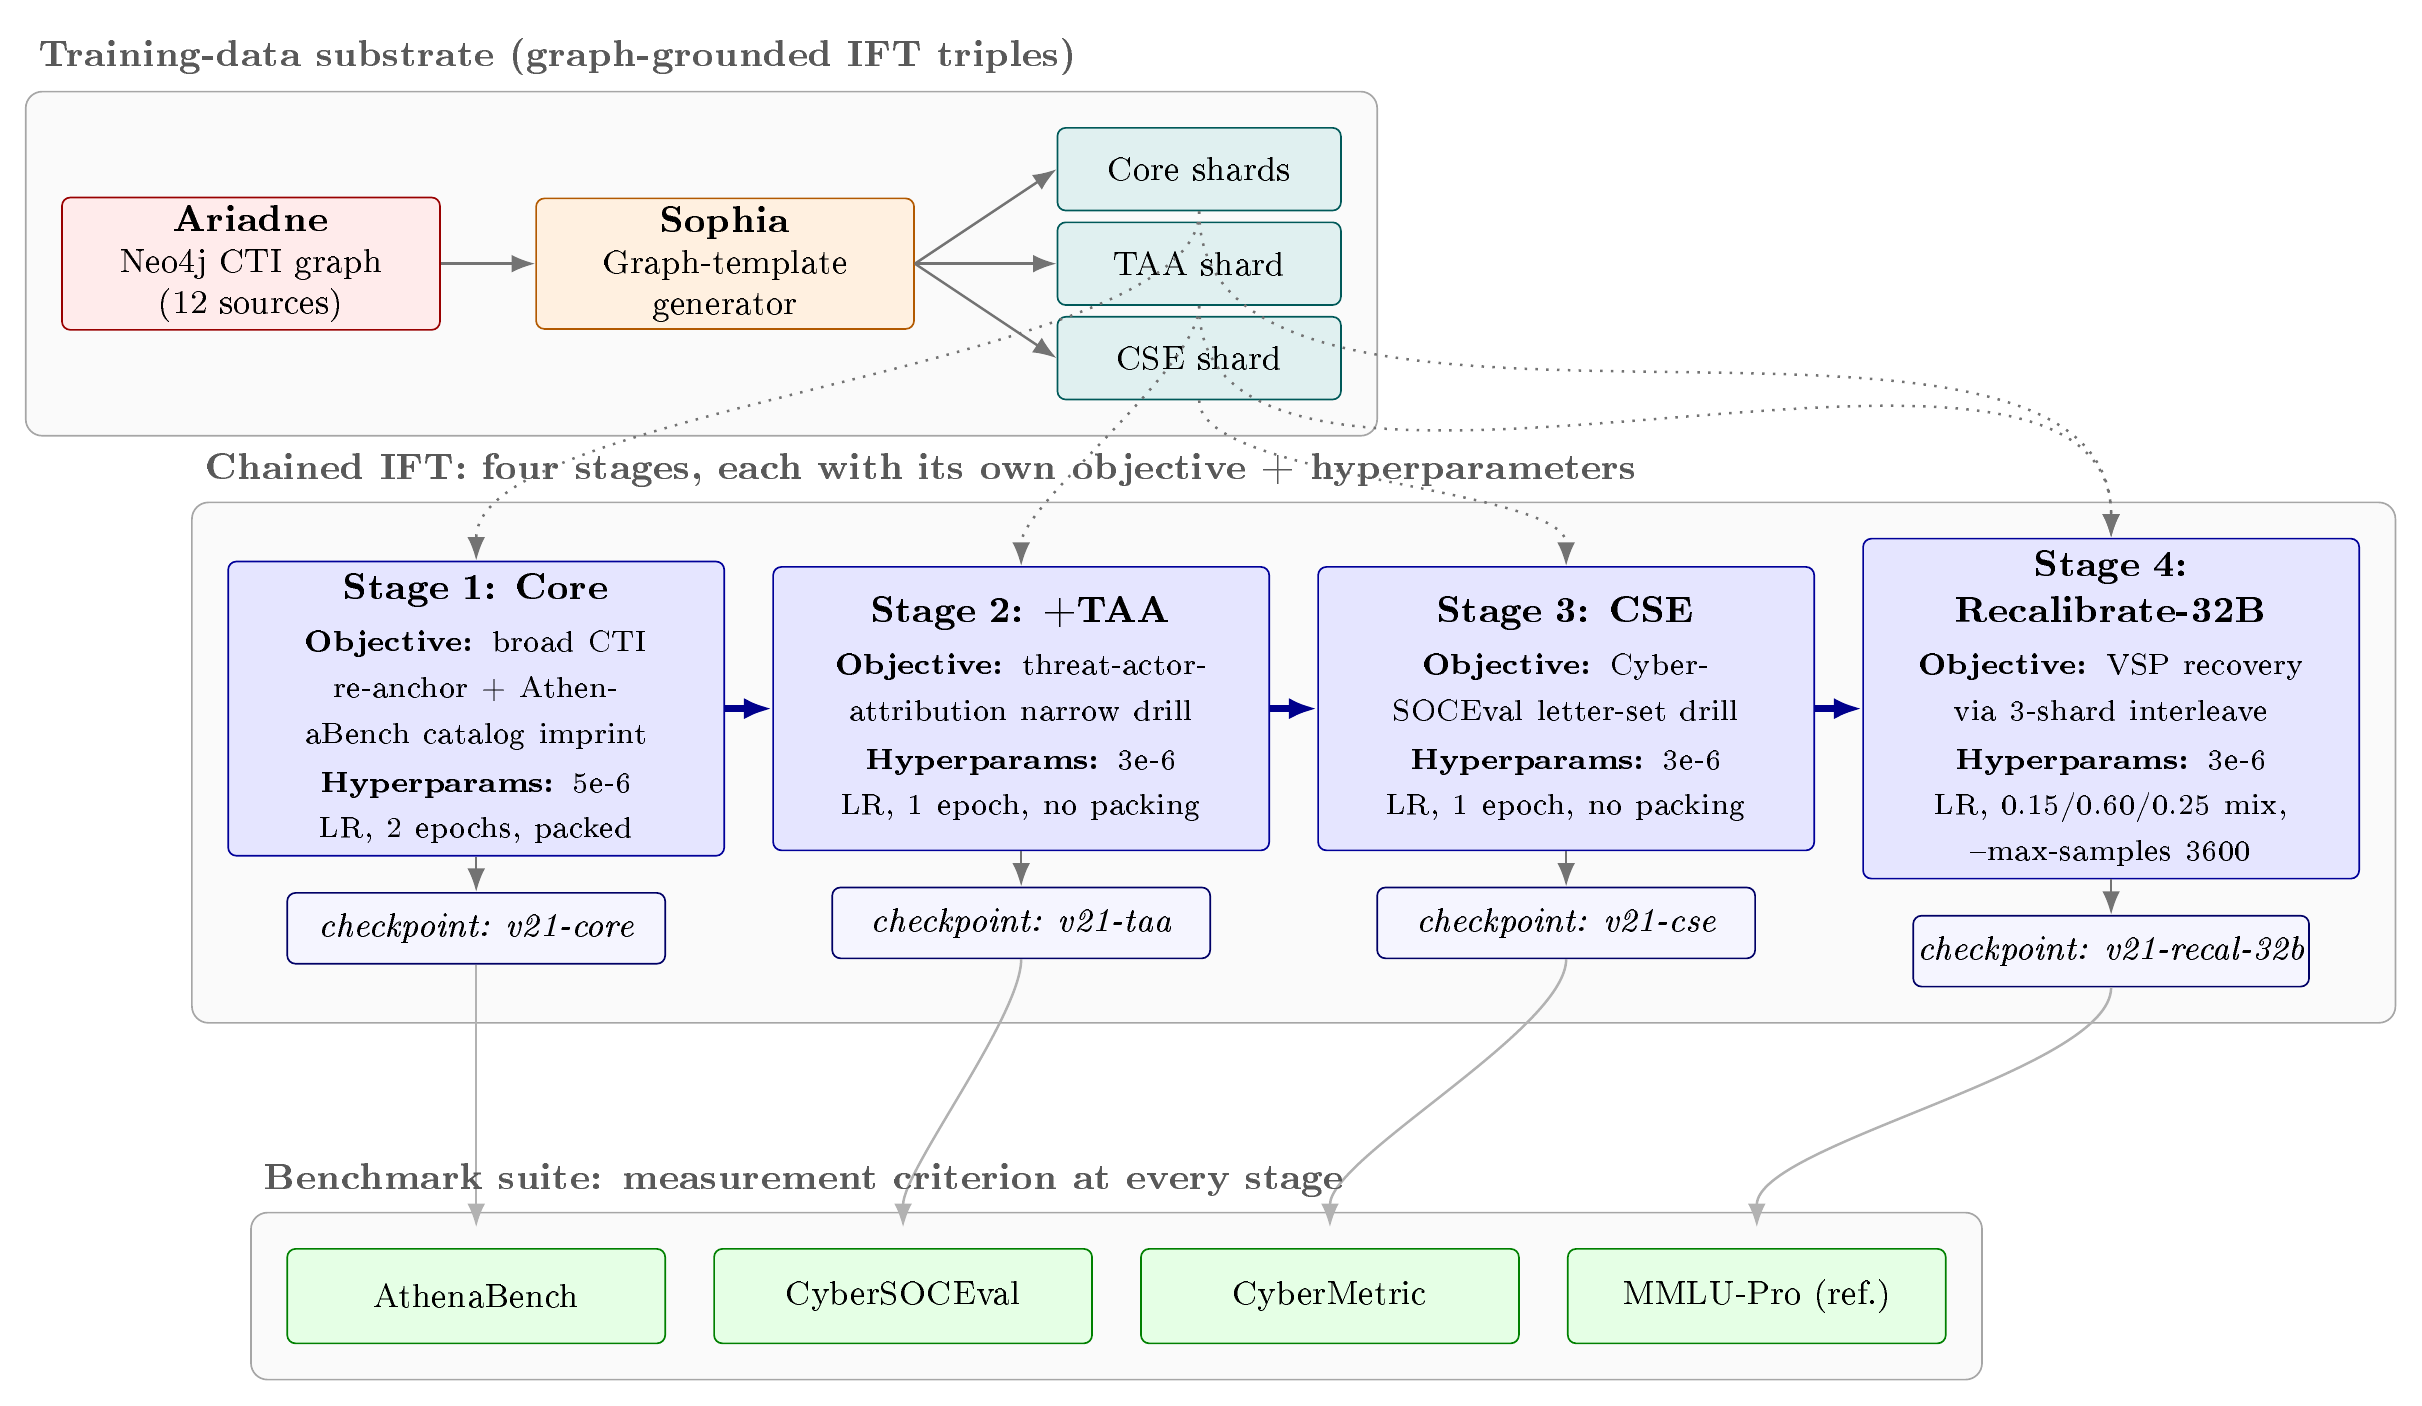
\includegraphics[width=\textwidth]{figures/glaukopis_chained_ift.png}
\caption{\textbf{The chained-IFT pattern.} Sophia compiles typed graph queries against Ariadne into Alpaca-format IFT triples, sharded into Core, TAA, and CSE manifests. The four-stage chain consumes these in order: each stage has its own objective (broad CTI re-anchor for Core, narrow drills for TAA and CSE, recalibration for Stage~4) and hyperparameters. Each stage pushes a cumulative checkpoint (\hfid{v21-core}, \hfid{v21-taa}, \hfid{v21-cse}, \hfid{v21-recal-32b}), each independently evaluable against the AthenaBench / CyberSOCEval / CyberMetric / MMLU-Pro suite, supporting per-stage ablation in addition to producing a single ship checkpoint.}
\label{fig:glaukopis-chained-ift}
\end{figure*}

\section{Background and Related Work}
\label{sec:ift-slm}

\textbf{IFT foundations.} Instruction fine-tuning (IFT) adapts a pretrained LLM on labeled (instruction, optional context, target) data, maximizing log-likelihood of the reference output \cite{wei2022flan,ouyang2022instructgpt}; it is one instantiation of supervised fine-tuning (SFT), and we use ``IFT'' following the cyber security literature. FLAN \cite{wei2022flan} established that instruction-following is a \emph{learnable} capability rather than a pure emergent of scale. InstructGPT \cite{ouyang2022instructgpt} introduced the staged SFT$\to$preference$\to$RLHF pipeline and showed that small instruction-tuned models can be preferred over much larger unaligned ones---the load-bearing argument for the small-model strategy here. FLAN-T5 \cite{chung2022flant5} scaled the instruction corpus to thousands of tasks and showed that instruction-data diversity and structure matter at least as much as parameter count, licensing the Glaukopis choice to invest in instruction-data structure at a fixed 32B budget.

\textbf{Chained IFT.} A recurring choice in modern post-training is to compose several IFT stages into a chain rather than a single monolithic tune: the output of each stage initializes the next, capabilities accumulate compositionally, and individual stages can be re-run when their data changes. Separating broad domain absorption from precise task behavior reduces destructive interference \cite{gururangan2020dontstop,ouyang2022instructgpt}; reasoning supervision is more effective layered on top of a model that already commands the domain vocabulary \cite{wei2022cot,levi2025toward}; and staging makes pipelines incrementally refreshable, which matters where source data turns over weekly. Glaukopis adopts a four-stage chain (Core, +TAA, CSE, Recalibrate-32B); the CyberPal.AI/SecKnowledge line operationalizes a related staging discipline on a different data pipeline \cite{levi2024cyberpal,levi2025toward}.

\textbf{Graph-grounded IFT.} The second refinement is on the data side: every triple is materialized by a typed query against an authoritative knowledge graph. This converges three lines: schema- and grammar-constrained generation (target outputs computed by executing queries against a reference database, not authored); knowledge-graph-grounded QA, where a typed traversal returns a subgraph rendered into a QA pair (CTI instantiations include \cite{fieblinger2024kg,wu2022opencykg,yu2024ctikg,zhao2024kctiaa,zhang2023cyberkg}); and expert-schema-driven IFT for cyber security \cite{levi2024cyberpal,levi2025toward}. Glaukopis combines all three: the Ariadne schema defines the typed substrate, every Sophia row is materialized by a Cypher query against the populated graph, and the driving templates are expert-authored CTI reasoning patterns.

\textbf{IFT and SLMs for cyber security.} Cyber security imposes heterogeneous schemas (CVE, CWE, CAPEC, ATT\&CK), evidence-grounded structured outputs, and rapid concept drift. SEvenLLM \cite{ji2024sevenllm} builds a bilingual instruction dataset and benchmark from incident reports; CyberBench \cite{liu2024cyberbench} provides cyber-specific instruction tasks and an evaluation suite. The closest neighbor is IBM's CyberPal.AI \cite{levi2024cyberpal}, which mines ATT\&CK, Sigma/SIEM rules, emulation plans, and threat reports into expert-defined instruction schemas; the SecKnowledge~2.0 follow-on \cite{levi2025toward} adds chain-of-thought enrichment, training 4--20B CTI-expert SLMs that rival larger general models. Glaukopis differs in three ways: every row is materialized from a typed CTI graph rather than synthesized; the SFT pass is a four-stage chain with explicit per-axis recovery; and the target is 32B---the smallest deployment-feasible scale at which the specialization/general-capability trade-off is acceptable for our workloads (Section~\ref{sec:results}). Such on-premises, air-gapped, low-latency deployment is exactly the regime in which well-targeted SLMs are most attractive \cite{levi2025toward}.

\section{Cyber Security LLM Benchmarks}
\label{sec:benchmarks}

General benchmarks (GLUE, MMLU, BIG-Bench) measure broad language understanding but were not designed to probe security workflows: they lack the structured schemas, evidence-grounded reasoning, and threat-current content that define CTI tasks, and---because MITRE, NVD, and public threat reports are heavily represented in pretraining corpora---static suites risk measuring recall of training data rather than reasoning \cite{alam2025athenabench}. The past two years have produced cyber-specific benchmarks spanning four overlapping families: knowledge (CyberMetric \cite{tihanyi2024cybermetric}, SecEval \cite{hu2024seceval}), secure-coding/offensive capability (Purple Llama CyberSecEval \cite{bhatt2023purplellama,bhatt2024cyberseceval2}, WMDP \cite{li2024wmdp}), applied CTI and SOC reasoning (CTIBench \cite{alam2024ctibench}, SEvenLLM-Bench \cite{ji2024sevenllm}, CyberSOCEval \cite{cybersoceval2025}), and dynamic/live-source suites (AthenaBench \cite{alam2025athenabench}).

No single benchmark suffices, so Glaukopis is evaluated against a portfolio: \textbf{AthenaBench} (a dynamic CTI suite drawing from live MITRE/NVD/CISA sources, with six tasks---CKT, RCM, VSP, TAA, RMS, ATE---that target staleness and contamination directly \cite{alam2025athenabench}); \textbf{CyberSOCEval} malware-analysis and threat-intel-reasoning suites (operational SOC reasoning over free-form narrative input \cite{cybersoceval2025}); \textbf{CyberMetric} at the 2K and 10K tiers (RAG-built, expert-validated MCQ giving statistically robust factual coverage \cite{tihanyi2024cybermetric}); and \textbf{MMLU-Pro} as a decoupled general-intelligence reference. AthenaBench is the training counterpart to Sophia/Ariadne: both derive from the same public sources but via independent pipelines, and Sophia's version/timestamp filters let training recency be aligned to AthenaBench's dynamic horizon to mitigate leakage \cite{cardei2025ift,alam2025athenabench}.

\section{Ariadne and Sophia: The Training-Data Pipeline}
\label{sec:cti-kg}

\textbf{Ariadne: the CTI knowledge graph.} Cyber threat intelligence is the collection, analysis, and dissemination of information about threats and adversaries to inform defensive decisions \cite{mcmillan2013gartner}. Ariadne is the populated Neo4j substrate that all downstream components (template generation, SFT, evaluation harness) consume as their single source of CTI facts; every fact in any training example must first exist as a node or edge in Ariadne, making the graph both the corpus's data layer and the harness's reference oracle. It ingests twelve public CTI sources spanning offensive technique catalogues (MITRE ATT\&CK \cite{strom2018mitreattck}, ENGAGE), attack-pattern and weakness taxonomies (CAPEC \cite{mitreCAPEC}, CWE \cite{mitreCWE}), defensive countermeasures (D3FEND, pinned to v1.4.0), vulnerability records (CVE 5.0 \cite{mitreCVE}, NVD CPE/CVSS), exploitation signals (CISA KEV, FIRST EPSS), detection content (Sigma), and weaponized-exploit evidence (ExploitDB, PoC-in-GitHub). The bounded catalogues (ATT\&CK, ENGAGE, CAPEC, CWE, KEV, D3FEND, Sigma) load in full; CVE, NVD, EPSS, ExploitDB, and PoC-in-GitHub are scoped to 2024 onward, keeping the graph at ${\sim}280$K nodes and ${\sim}480$K edges---large enough for multi-hop cross-schema reasoning, small enough for practical single-instance query latency.

The populator is idempotent (\texttt{MERGE} against per-node uniqueness constraints on \hfid{stix_id}, CVE/CWE/D3FEND IDs, etc.), so re-runs never duplicate. Three refresh policies apply: \emph{always-refresh} (EPSS, current-year NVD, both daily), \emph{skip-if-cached HTTPS} (CAPEC, CWE, KEV, D3FEND), and \emph{skip-if-cached Git} (ATT\&CK, ENGAGE, CVE, Sigma, ExploitDB, PoC-in-GitHub); production runs a nightly cron that picks up daily EPSS/NVD churn while leaving static catalogues untouched. Construction proceeds in a fixed dependency order---framework nodes first, then the vulnerability surface, then the weaponized-exploit layer---so cross-framework edges (CVE$\to$CWE root-cause, CWE$\to$CAPEC$\to$ATT\&CK pivots, ATT\&CK$\to$Mitigation, D3FEND$\leftrightarrow$ATT\&CK) always have both endpoints present. Every SFT row is traceable to specific graph identifiers, which resolve to public-source rows by their natural keys---the basis of the chained-IFT auditability claim.

\textbf{Sophia: graph-template-driven generation.} Sophia (\hfid{tmpl_gen}) compiles declarative CTI reasoning patterns into Alpaca triples by issuing Cypher queries against Ariadne and binding returned nodes, properties, and relationships into (instruction, input, output) records \cite{cardei2025ift}. Because every template resolves to typed traversals over named-key constraints, each triple is grounded in specific elements citable by natural key (e.g., \hfid{CVE-2024-12345}, \texttt{T1059.003}, \hfid{CAPEC-66}). A three-step wrapper (\hfid{make_dataset.sh}) drives it: \texttt{docx2json} extracts templates from \texttt{.docx}/JSON authoring formats; \texttt{tmpl2triples} opens a Bolt connection, issues the implied queries, and emits per-template triples with a \hfid{_results-report.json} summary of failures; \texttt{triples2alpaca} merges them into one dataset. A representative template binds a node to an alias and emits its properties:

\begin{quote}\scriptsize\ttfamily\sloppy\setlength{\rightskip}{0pt plus 2em}\noindent
M.1 Instruction: You are a cyber security expert\ldots\\
Question: Explain ATT\&CK technique \{ap:attack-pattern.name\} (\{ap.id\}) and how it is used.\\
Answer: Technique \{ap.name\} (\{ap.id\}) is described as: \{ap.description\}. Commonly observed across \{ap.x\_mitre\_platforms\}.
\end{quote}

\noindent The full language adds relationship traversal (\verb|{v.rel>Type.prop}|), filters with any/all semantics on list-valued properties, list-comprehension expansions, invisible binding sections, and source-disambiguating prefixes (\verb|attck#attack-pattern| vs.\ \verb|capec#attack-pattern|) \cite{cardei2025ift}. Its scientific advantages over LLM-authored instruction sets are \emph{ground-truth faithfulness} (answers computed from an authoritative graph), \emph{explicit coverage control}, \emph{rich hard negatives} (mitigations that do \emph{not} address a technique, etc.), \emph{auditability} (each row re-derivable by re-running its Cypher), and \emph{incremental refresh} via version/date filters \cite{cardei2025ift,alam2025athenabench}. Conceptually, where CyberPal synthesizes instructions from unstructured sources using LLMs and experts \cite{levi2024cyberpal,levi2025toward}, Sophia uses a declarative template language over a typed graph to generate strongly grounded, precisely controllable triples. Figure~\ref{fig:sophia-flow} shows the end-to-end flow from the upstream public CTI sources through the Sophia generator and the v21 curation pipeline to the Alpaca-format IFT shards consumed by the chained-IFT stages.

\begin{figure*}[t]
\centering
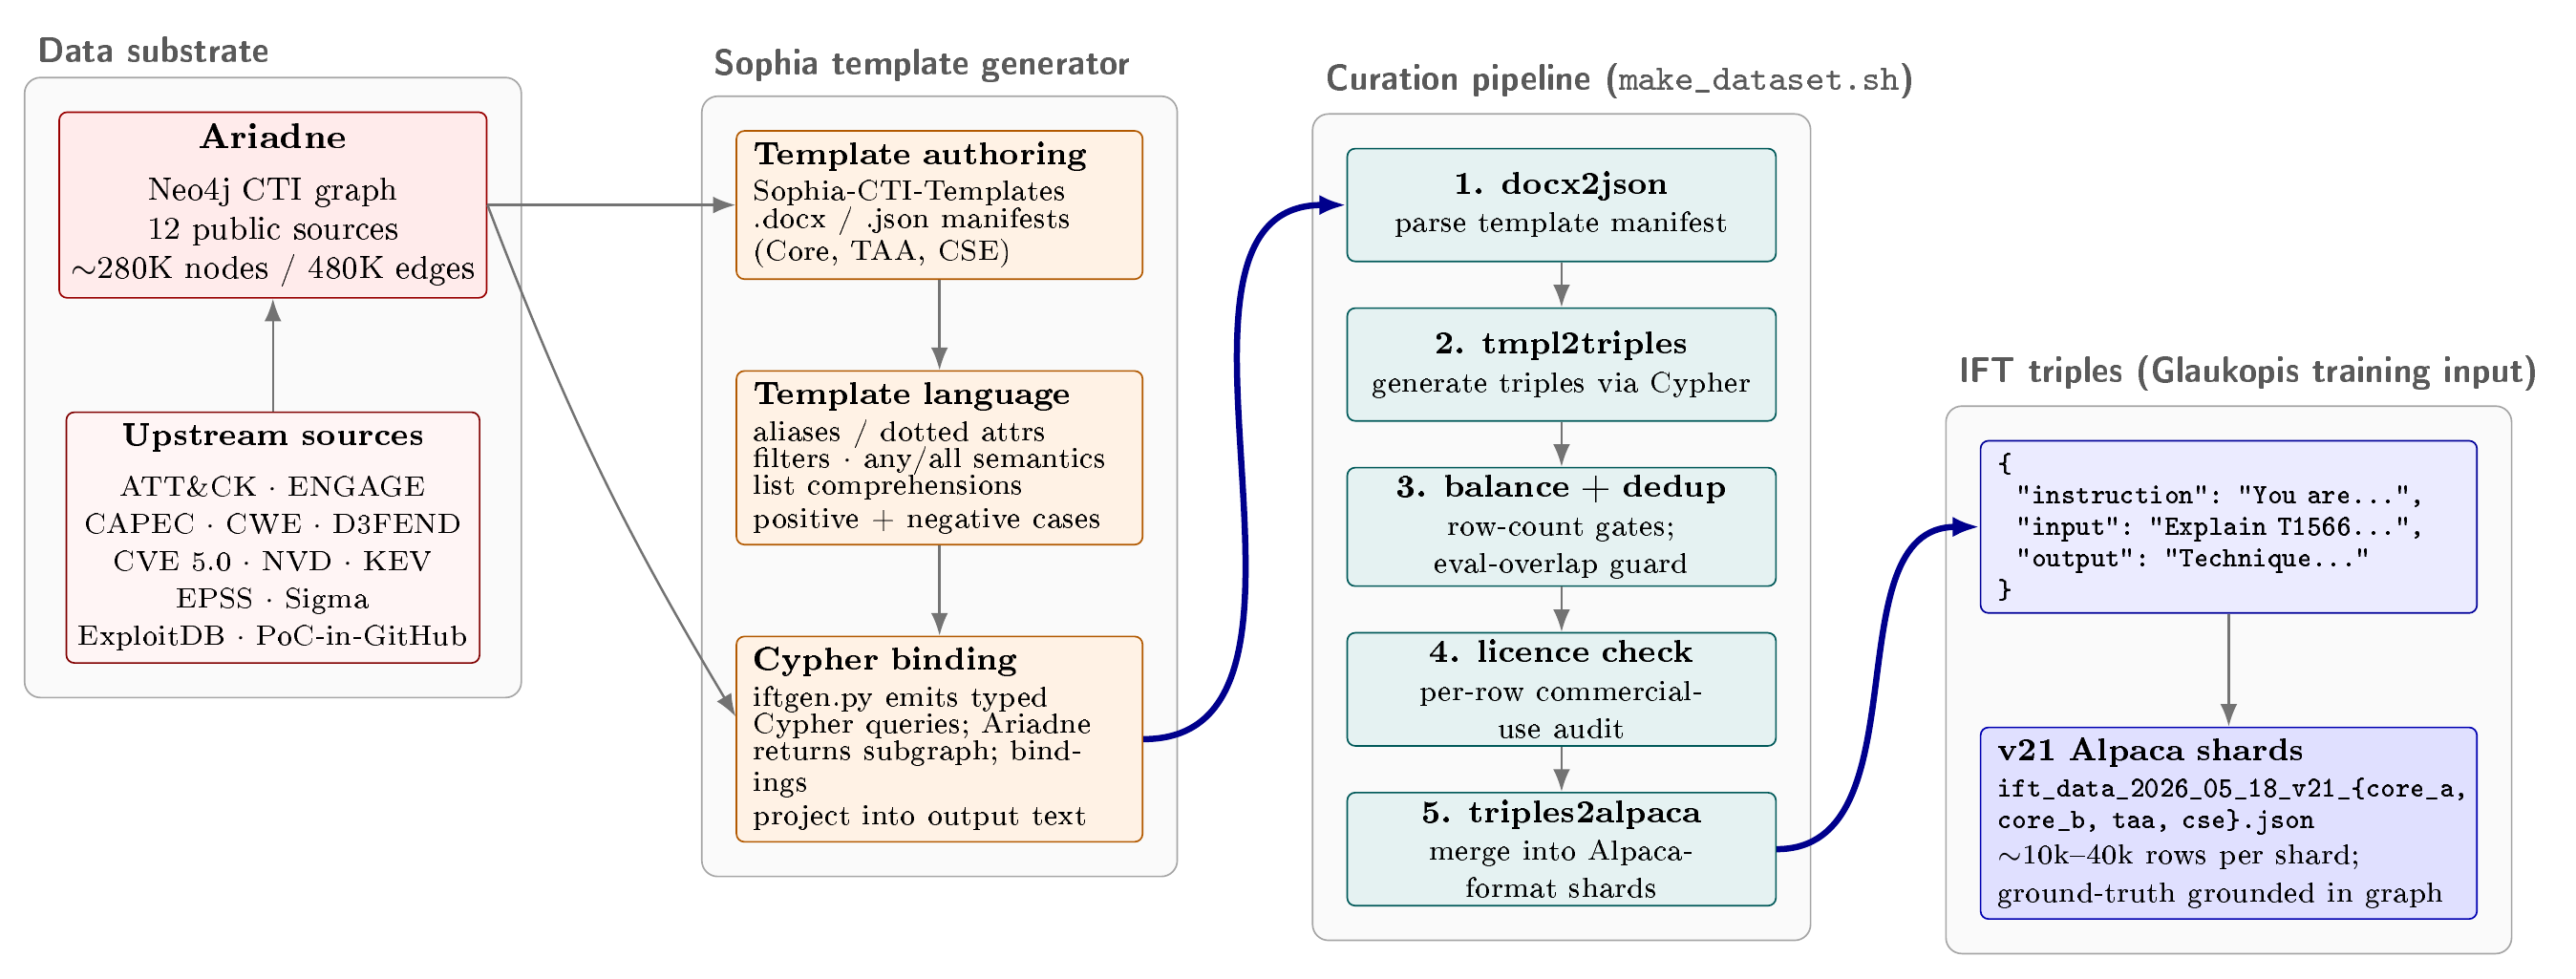
\includegraphics[width=\textwidth]{figures/glaukopis_sophia_flow.png}
\caption{\textbf{Sophia template generation and v21 data flow.} The upstream public CTI sources (left) are ingested into the Ariadne Neo4j graph. Sophia (centre-left) authors templates in three artefacts---template manifests (.docx/.json), the template language, and the Cypher binding step in \texttt{iftgen.py}---each of which compiles graph queries into natural-language output. The v21 curation pipeline (\hfid{make_dataset.sh}, centre-right) runs five steps in order: parse the template manifest, generate triples via Cypher, balance and dedup the corpus against the row-count gates and the eval-overlap guard (Section~\ref{sec:open-challenges}), check per-row licence compliance, and merge the per-template files into Alpaca-format shards. The output (right) is the set of Alpaca-format IFT shard files (\texttt{ift\_data\_2026\_05\_18\_v21\_\{core\_a, core\_b, taa, cse\}.json}) consumed directly by the chained-IFT training stages (Section~\ref{sec:glaukopis}).}
\label{fig:sophia-flow}
\end{figure*}

\section{Glaukopis: The Chained-IFT Pipeline}
\label{sec:glaukopis}

Glaukopis produces the Athena-CTI-LLM family via template-based chained IFT: Ariadne drives Sophia (Section~\ref{sec:cti-kg}); Sophia emits IFT triples sharded into purpose-built datasets; those feed a four-stage chain; and each resulting checkpoint is evaluated against the portfolio of Section~\ref{sec:benchmarks}.

\textbf{The v21 vintage.} The active vintage is \textbf{v21} (template directory \hfid{tmpl_gen/templates/05182026/}), which projects Ariadne through three template manifests---Core, TAA, and CSE---into four production training shards plus three matched validation shards. All shards are template-baked and therefore architecture-independent: one set of seven JSON files feeds every base-model port. v21 is a strict reproducibility experiment forked from v18.1: the manifests, row-count gates, and per-stage count limits are \texttt{shasum}-verified byte-identical to v18.1, with only dataset names and Hugging Face push targets changed. The sign-off gate was that the post-Core checkpoint land within $\pm1.5$ points of the v18.1 Core peak on every axis; Total Score landed inside the band but two sub-scores (ATE, RCM) drifted, with the same shape seen in the intermediate v19/v20 vintages. Since the recipe-side inputs are byte-identical, the most parsimonious explanation is data-build non-determinism in the substrate sampler, dedup tiebreaks, and shuffle seeding inside \hfid{make_dataset.sh}---making seed-pinning the next-vintage direction. Carrying byte-identical templates and gates forward across vintages isolates recipe drift from data-layer drift as separable failure modes, which is itself a contribution.

The same recipe ports byte-identically across five base architectures (Table~\ref{tab:base-models}); any axis-level differences are therefore attributable to base-model differences rather than training-data drift. The Qwen3-MoE port additionally exercises a thinking-on/off A/B at serve time.

\begin{table*}[t]
\centering
\caption{Baseline instruct models targeted by the v21 architecture ports. The dense Qwen-2.5-32B-Instruct is the canonical Stage-0 base for the ship checkpoint reported in Section~\ref{sec:results}; the other four are cross-architecture ports of the same v21 chain.}
\label{tab:base-models}
\small
\setlength{\tabcolsep}{4pt}
\begin{tabular}{p{4.8cm} l l l}
\hline
\textbf{Canonical HF identifier} & \textbf{Family} & \textbf{Architecture} & \textbf{Role in v21} \\
\hline
\hfid{Qwen/Qwen2.5-32B-Instruct}             & Qwen 2.5             & 32B dense          & Canonical Stage-0 base (ship) \\
\hfid{Qwen/Qwen2.5-14B-Instruct}             & Qwen 2.5             & 14B dense          & Cross-architecture port \\
\hfid{Qwen/Qwen3-30B-A3B-Thinking-2507}      & Qwen 3 Thinking      & 30B MoE (A3B)      & MoE / thinking-mode port \\
\hfid{meta-llama/Meta-Llama-3.1-8B-Instruct} & Llama 3.1            & 8B dense           & Cross-architecture port \\
\hfid{fdtn-ai/Foundation-Sec-8B-Instruct}    & Foundation-Sec       & 8B dense           & Security-specialized base (Cisco) \\
\hline
\end{tabular}
\end{table*}

\textbf{The four-stage SFT chain.} Each stage runs standard SFT on next-token cross-entropy; the chain consumes seven Sophia shards. \textbf{Core-A} is a broad re-anchor mix (knowledge-base, MCQ, TAA, SOC, CyberMetric-style, mitigation, yes/no families); \textbf{Core-B} is an AthenaBench catalog drill (RMS, ATE, VSP, RCM); \textbf{TAA} is a narrow TAA-Classic drill; \textbf{CSE} is a CyberSOCEval letter-set drill; three matched validation shards hold out 50 rows per shortname.

\emph{Stage 1 (Core)} runs two phases, pushing only the final merged checkpoint. Phase~A re-establishes broad instruction-following on Core-A plus a general mix (Tülu-3 SFT, Alpaca-English) at seq-len 8\,192, packing on, LR $1\times10^{-5}$, effective batch 16. Phase~B drills Core-B at seq-len 16\,384, packing off (so long structured outputs are not truncated), LR $5\times10^{-6}$, effective batch 8, imprinting precise AthenaBench task structure \cite{alam2025athenabench,chung2022flant5,gururangan2020dontstop}. \emph{Stage 2 (+TAA)} trains the Core checkpoint on TAA alone (seq-len 4\,096, packing on, LR $5\times10^{-6}$, batch 16), hardening TAA-Classic without disturbing catalog skills. \emph{Stage 3 (CSE)} trains the +TAA checkpoint on CSE at the same settings, targeting the CyberSOCEval suites \cite{cybersoceval2025}; this reliably trades ${\sim}10$ points of VSP for the CyberSOCEval lift. \emph{Stage 4 (Recalibrate, ship)} is an off-plan three-shard interleaved touch-up over Core-A/Core-B/TAA that recovers the VSP regression without losing Stage~3 gains. At 14B a single recipe (LR $1\times10^{-6}$, $0.25/0.40/0.35$ mix, \hfid{--max-samples 2400}) cleanly recovers VSP; at 32B the same recipe sits at the \hfid{adamw_8bit} noise floor and drifts VSP the wrong way, so it is re-tuned (LR $3\times10^{-6}$, Phase-B-heavy $0.15/0.60/0.25$ mix, \hfid{--max-samples 3600}) via LlamaFactory's \hfid{interleave_under} strategy. All stages share bf16, DeepSpeed ZeRO-3, the \hfid{adamw_8bit} optimizer (mandatory at 32B), Liger kernels, and gradient checkpointing; the canonical target is 8$\times$H100-80GB, with effective batch held constant across topologies by auto-scaling gradient accumulation.

The four-stage structure is the load-bearing element: Stages~1A/1B separate broad absorption from structured-task imprinting, Stages~2/3 drill specific axes without re-perturbing prior skills, and Stage~4 recovers regressed axes through controlled interleaving. Because every stage pushes a checkpoint and consumes a specific shard, any axis-level regression is attributable to a specific stage and addressable by re-running only the affected stages.

\textbf{Evaluation harness.} Each checkpoint is served via vLLM (OpenAI-compatible) and scored on AthenaBench (six CTI tasks), CyberSOCEval (malware + threat-intel), CyberMetric (2K, 10K), and MMLU-Pro; the same alias-keyed harness scores public baselines through hosted providers. Per-task token and wall-clock usage is captured so cost is reported alongside accuracy. The stage$\to$suite mapping is deliberate: Core-B exercises RMS/ATE/VSP/RCM, Stage~2 exercises TAA, Stage~3 exercises CyberSOCEval, and Core-A exercises CyberMetric and the MCQ axis; MMLU-Pro is run separately as a forgetting diagnostic, not an optimization target.

\section{Results}
\label{sec:results}

We evaluate the v21 vintage against the portfolio of Section~\ref{sec:benchmarks}. All numbers come from a single harness run (sweep dated 2026-05-24), using the same vLLM stack for local checkpoints and the same hosted endpoints for public baselines.

\textbf{Three averaging schemes.} Because the CTI benchmarks differ in internal structure (AthenaBench has six tasks, CyberSOCEval two, CyberMetric two tiers), the choice of aggregation visibly changes the leaderboard, so we report three. \emph{Avg CTI Benchmark} is the unweighted mean of three per-benchmark summaries (each benchmark equal weight)---our cross-benchmark metric, closest to published leaderboards. \emph{Avg CTI Test} is the unweighted mean across the ten individual CTI tests, the most apples-to-apples cross-architecture view. \emph{Avg Total (w/MMLU-Pro)} extends the per-test average with MMLU-Pro to quantify how much general capability each run trades away---a \textit{general-knowledge erosion} diagnostic, not an optimization target. Cost is measured uniformly: published per-1K-token rates for hosted checkpoints, and wall-clock at \$2.50/GPU-hour on a 2$\times$H100 host for local vLLM checkpoints.

\textbf{Headline comparison.} Table~\ref{tab:results-headline} compares the v21 ship checkpoint against its base and six frontier references. Three observations: (1) chained SFT adds \textbf{7.3 points} of Avg CTI Benchmark over Qwen-2.5-32B-Instruct ($59.0\to66.3$) and 13.3 on Avg CTI Test ($49.6\to62.9$), with the largest single-axis lift on AthenaBench combined ($44.2\to66.5$, $+22.3$). (2) The ship sits within 4--7 points of the leading frontier models (GPT-5.5 72.9, DeepSeek-V4-Pro 70.4, Gemini-3-Flash-Preview 69.8), exceeds Gemini-2.5-Flash (63.4), and runs even with DeepSeek-V3.2-Exp (66.0) despite the parameter gap. (3) General-knowledge erosion is real but graded and not unique to Glaukopis: MMLU-Pro drops $69.0\to57.4$ ($-11.6$), reflecting the known cost of specialization; we report it as a diagnostic rather than optimizing against it.

The two Stage-4 variants share the same Stage-3 parent and differ only in recipe. On headline aggregates they are within 0.5 points; the deciding factor is per-axis VSP recovery: \hfid{v21-recal-32b} restores VSP to 77.8 vs.\ \hfid{v21-recalibrate}'s 75.7, which is precisely what Stage~4 is for at 32B. \hfid{v21-recal-32b} is therefore the ship checkpoint.

\begin{table*}[t]
\centering
\caption{Headline results: Glaukopis v21 ship checkpoint vs.\ base model and frontier reference points. Three averages are reported per the schemes defined in Section~\ref{sec:results}: \textbf{Avg CTI Bench} (3 benchmarks, equal weight), \textbf{Avg CTI Test} (10 CTI tests, equal weight), and \textbf{Avg Total (w/MMLU)} (10 CTI tests plus MMLU-Pro). All numbers from the 2026-05-24 evaluation sweep. AB Avg II is the AthenaBench composite using the 50/50 TAA Classic+Canonical blend.}
\label{tab:results-headline}
\small
\setlength{\tabcolsep}{4pt}
\begin{tabular}{lcccccccc}
\hline
\textbf{Model} & \textbf{Type} & \textbf{Avg CTI} & \textbf{Avg CTI} & \textbf{Avg Total} & \textbf{AB Avg} & \textbf{CSE} & \textbf{CM} & \textbf{MMLU-} \\
               &               & \textbf{Bench}   & \textbf{Test}    & \textbf{(w/MMLU)}  & \textbf{II}    & \textbf{comb} & \textbf{avg} & \textbf{Pro} \\
\hline
GPT-5.5                                  & Frontier  & 72.9 & 73.5 & 76.9 & 77.0 & 48.3 & 93.3 & 88.3 \\
DeepSeek-V4-Pro                          & OS-PT     & 70.4 & 67.9 & 69.6 & 67.2 & 52.2 & 91.8 & 79.1 \\
Gemini-3-Flash-Preview                   & Frontier  & 69.8 & 68.4 & 71.7 & 69.3 & 48.1 & 92.1 & 89.2 \\
GPT-5.2 (reasoning=medium)               & Frontier  & 67.5 & 65.0 & 67.0 & 63.8 & 46.8 & 91.8 & 81.3 \\
DeepSeek-v3.2-Exp                        & OS-PT     & 66.0 & 62.2 & 63.9 & 59.0 & 47.2 & 91.7 & 82.5 \\
\textbf{v21-recal-32b (ship)}            & SFT       & \textbf{66.3} & \textbf{62.9} & \textbf{62.8} & \textbf{66.5} & 42.6 & 89.8 & 57.4 \\
v21-cse                                  & SFT       & 65.8 & 62.4 & 62.2 & 66.6 & 42.0 & 88.8 & 54.2 \\
v21-recalibrate (14B-recipe)             & SFT       & 65.9 & 62.4 & 62.2 & 65.9 & 42.4 & 89.2 & 54.6 \\
Gemini-2.5-Flash                         & Frontier  & 63.4 & 57.9 & 59.8 & 53.1 & 46.2 & 91.0 & 82.1 \\
v21-core                                 & SFT       & 62.6 & 61.6 & 63.2 & 67.2 & 31.1 & 89.6 & 59.2 \\
v21-taa                                  & SFT       & 62.0 & 61.7 & 63.7 & 66.9 & 29.8 & 89.4 & 58.2 \\
Qwen2.5-32B-Instruct (base)              & Instruct  & 59.0 & 49.6 & 49.3 & 44.2 & 42.6 & 90.2 & 69.0 \\
\hline
\end{tabular}
\end{table*}
\textbf{Per-stage ablation.} Because the chain pushes a checkpoint after every stage, per-stage contributions are directly measurable (Table~\ref{tab:results-per-stage}). Stage~1 (Core) does most of the catalog work---ATE $18.2\to67.2$, RMS $7.6\to63.8$, RCM $59.5\to69.8$. Stage~2 introduces Canonical-TAA capability (TAA Canonical $2.0/18.4\to36.8$). Stage~3 lifts CyberSOCEval ($31.1\to42.0$) at the expected VSP cost ($83.1\to78.9$). Stage~4 is recovery, not novel capability: it re-aligns VSP (77.8) and stabilizes CyberSOCEval (42.6) rather than developing new capability.

\begin{table*}[t]
\centering
\caption{Per-stage AthenaBench breakdown for the Qwen-2.5-32B v21 chain (combined-form scores where multiple forms are released). Stage 1 (Core) does most of the AthenaBench-catalog work; Stage 2 introduces Canonical TAA; Stage 3 lifts CyberSOCEval; Stage 4 recovers VSP without losing prior gains.}
\label{tab:results-per-stage}
\small
\begin{tabular}{lcccccccc}
\hline
\textbf{Checkpoint} & \textbf{CKT} & \textbf{ATE} & \textbf{RCM} & \textbf{RMS} & \textbf{VSP} & \textbf{TAA Cl.} & \textbf{TAA Can.} & \textbf{AB II} \\
\hline
Qwen2.5-32B-Instruct (base) & 52.9 & 18.2 & 59.5 & 7.6  & 78.8 & 48.0 & 2.0  & 44.2 \\
v21-core                    & 72.9 & 67.2 & 69.8 & 63.8 & 83.1 & 46.5 & 18.4 & 67.2 \\
v21-taa                     & 75.4 & 63.4 & 69.0 & 62.9 & 83.5 & 47.0 & 36.8 & 66.9 \\
v21-cse                     & 72.5 & 63.4 & 67.7 & 63.7 & 78.9 & 53.5 & 3.4  & 66.6 \\
\textbf{v21-recal-32b}      & 75.5 & 65.8 & 67.1 & 62.5 & 77.8 & 50.5 & 3.4  & \textbf{66.5} \\
\hline
\end{tabular}
\end{table*}
\textbf{Cross-architecture ports.} The same recipe ports byte-identically to four other bases (Table~\ref{tab:results-architectures}). Recipe transfer scales with base size: the 14B and 32B dense Qwen ports lift +13.5/+13.3 on Avg CTI Test, Llama-3.1-8B +7.3, the Qwen3-MoE port +6.0, and Foundation-Sec-8B only +0.4 (already a security-specialized base). The Qwen3-MoE port leads on MMLU-Pro among SFT'd checkpoints (53.0) but is more expensive to serve and loses on the CTI averages; the dense Qwen-2.5-32B port is the most CTI-capable and most efficient ship. MMLU-Pro regression is largest at smaller scales (8B: 17.6--20.6; 14B: 13.9; 32B: 11.6; MoE: 24.6).

\begin{table*}[t]
\centering
\caption{Cross-architecture v21 ports. \emph{Best v21}: highest-scoring SFT checkpoint for that base architecture on Avg CTI Benchmark Score. \textbf{Avg CTI Bench} and \textbf{Avg CTI Test} are the per-benchmark and per-test schemes defined in Section~\ref{sec:results}. \emph{$\Delta$ test} and \emph{$\Delta$ MMLU}: absolute differences between the best SFT checkpoint and the corresponding instruct base on Avg CTI Test and MMLU-Pro respectively. The Qwen-2.5-32B dense port is the cross-architecture optimum on CTI; the Qwen3-MoE port leads on MMLU-Pro among SFT'd checkpoints but is more expensive to serve and benchmark.}
\label{tab:results-architectures}
\small
\setlength{\tabcolsep}{4pt}
\begin{tabular}{llccccc}
\hline
\textbf{Base architecture}  & \textbf{Best v21 checkpoint} & \textbf{Avg CTI} & \textbf{Avg CTI} & \textbf{$\Delta$ test} & \textbf{MMLU-} & \textbf{$\Delta$ MMLU} \\
                            &                              & \textbf{Bench}   & \textbf{Test}    & \textbf{vs.\ base}     & \textbf{Pro}   & \textbf{vs.\ base}     \\
\hline
Qwen2.5-32B-Instruct        & v21-recal-32b   & \textbf{66.3} & \textbf{62.9} & +13.3 & 57.4 & $-$11.6 \\
Qwen2.5-14B-Instruct        & v21-recalibrate & 62.3 & 59.6 & +13.5 & 50.2 & $-$13.9 \\
Qwen3-30B-A3B-Thinking-2507 & v21-cse         & 63.4 & 60.9 &  +6.0 & 53.0 & $-$24.6 \\
Foundation-Sec-8B-Instruct  & v21-recalibrate & 53.8 & 53.2 &  +0.4 & 25.6 & $-$17.6 \\
Llama-3.1-8B-Instruct       & v21-recalibrate & 50.5 & 50.8 &  +7.3 & 27.7 & $-$20.6 \\
\hline
\end{tabular}
\end{table*}
\textbf{Cost.} On a full-suite pass, the v21 ship costs \$2.83 (Table~\ref{tab:results-cost}). The most expensive proprietary model, Gemini-3-Flash-Preview, costs \$1{,}154.13 ($408\times$); GPT-5.5 \$508.13 ($180\times$); Gemini-2.5-Flash---which the ship beats on every CTI average---\$166.24 ($59\times$); DeepSeek-V4-Pro \$126.40 ($45\times$). The cheapest API-priced references (DeepSeek-V3 family, \$11--14) are still 4--5$\times$ the locally-served ship despite far larger parameter counts. Normalized by capability, the ship sits at \$0.043 per Avg-CTI-Bench point---an order of magnitude below the cheapest API frontier reference (\$0.17) and ${\sim}60\times$ below the cheapest proprietary one (\$2.62). Two reasons make this decisive: regulated SOCs cannot send telemetry to a third-party API, and even where allowed, frontier per-evaluation cost compounds across analyst workloads. A 32B local checkpoint that closes most of the gap changes the calculus from ``frontier or nothing'' to ``frontier when allowed, on-premises 32B otherwise.''

\begin{table*}[t]
\centering
\caption{Full-suite evaluation cost (\$USD) for the v21 ship checkpoint vs.\ frontier reference points and Glaukopis intermediate stages. Cost is the sum of per-benchmark cost across AthenaBench, CyberSOCEval, CyberMetric 2K+10K, and MMLU-Pro. Local checkpoints are billed at \$2.50/GPU-hr on 2$\times$H100; hosted-API checkpoints are priced by published per-1K-token rate. \emph{Cost ratio} is full-suite cost divided by the v21 ship cost (\$2.83); \emph{Avg CTI Bench} is reproduced from Table~\ref{tab:results-headline} for cost-vs-capability context.}
\label{tab:results-cost}
\small
\setlength{\tabcolsep}{4pt}
\begin{tabular}{lccccc}
\hline
\textbf{Model} & \textbf{Billing} & \textbf{Full-suite cost} & \textbf{Cost} & \textbf{Avg CTI} & \textbf{\$/CTI} \\
               & \textbf{basis}   & \textbf{(USD)}            & \textbf{ratio} & \textbf{Bench} & \textbf{point} \\
\hline
\multicolumn{6}{l}{\textit{Frontier proprietary (API-priced)}} \\
Gemini-3-Flash-Preview            & API tokens & 1{,}154.13 & 408$\times$ & 69.8 & 16.5 \\
GPT-5.5 (reasoning=medium)        & API tokens &    508.13 & 180$\times$ & 72.9 &  6.97 \\
GPT-5.2 (reasoning=medium)        & API tokens &    209.67 &  74$\times$ & 67.5 &  3.11 \\
Gemini-2.5-Flash                  & API tokens &    166.24 &  59$\times$ & 63.4 &  2.62 \\
\multicolumn{6}{l}{\textit{Frontier open-weights (API-priced)}} \\
DeepSeek-V4-Pro                   & API tokens &    126.40 &  45$\times$ & 70.4 &  1.80 \\
DeepSeek-V3.1-Terminus            & API tokens &     14.33 &   5$\times$ & --- & --- \\
DeepSeek-V3.2-Exp                 & API tokens &     11.24 &   4$\times$ & 66.0 &  0.17 \\
\multicolumn{6}{l}{\textit{Glaukopis 32B and base (locally served)}} \\
Qwen2.5-32B-Instruct (base)       & 2$\times$H100 &    10.67 & 3.8$\times$ & 59.0 & 0.18 \\
\textbf{v21-recal-32b (ship)}     & 2$\times$H100 & \textbf{2.83} & \textbf{1.0$\times$} & \textbf{66.3} & \textbf{0.043} \\
v21-recalibrate (14B-recipe)      & 2$\times$H100 &     2.51 & 0.9$\times$ & 65.9 & 0.038 \\
v21-cse                           & 2$\times$H100 &     2.18 & 0.8$\times$ & 65.8 & 0.033 \\
v21-core                          & 2$\times$H100 &     2.88 & 1.0$\times$ & 62.6 & 0.046 \\
v21-taa                           & 2$\times$H100 &     2.73 & 1.0$\times$ & 62.0 & 0.044 \\
\hline
\end{tabular}
\end{table*}
\section{Open Challenges and Conclusion}
\label{sec:open-challenges}

Several directions follow from the v21 results. The most direct is layering a \textbf{reinforcement-learning phase with verifiable CTI rewards} on top of the IFT chain---essentially a Stage~5 ``Verify''---scoring completions against Ariadne-derived gold answers for closed-form tasks (RCM, VSP) or rubrics for open-ended ones (RMS, TAA). Minerva \cite{alam2026minerva} (by a co-author) shows that RL with verifiable CTI rewards delivers gains pure IFT leaves on the table, echoing the RL-style refinement in SecKnowledge~2.0 \cite{levi2025toward}. A second direction is \textbf{larger base models} (70--72B) to mitigate the parameter-count-graded general-knowledge erosion documented above, at roughly $2\times$ the serving footprint. Further directions include \textbf{embedding-similarity dedup} for paraphrastic leakage beyond the n-gram guard, \textbf{hybrid template/LLM generation} for surface diversity while preserving correctness, \textbf{CoT enrichment} of Sophia rows \cite{levi2025toward}, and \textbf{operational evaluation} (prompt-injection robustness, latency, SIEM/SOAR integration) \cite{hu2024seceval,liu2024cyberbench,alam2025athenabench}.

We address contamination explicitly. The v21 build distinguishes \emph{verbatim} contamination (eval text reproduced in a training row---bad) from \emph{structural} overlap (training and eval rows independently derived from the same public graph---accepted). A single guard, \hfid{dedup_against_evals.py}, runs once per shard at build time: it indexes the union of $n{=}13$ word-grams across every AthenaBench/CTIBench/CyberMetric/CyberSOCEval eval file, then flags any SFT row sharing a 13-gram (\hfid{--hit-threshold 1}) and filters any row reaching 50 shared 13-grams against a single eval row (\hfid{--drop-threshold 50})---the same window used by OLMo/Pythia/Llama decontamination. Paraphrastic leakage, which n-gram dedup misses, is addressed structurally: Sophia templates are generated from the graph, not from eval text, so overlap is only possible when both rows independently describe the same graph fact. The guard is enforced per shard (a non-zero exit skips dataset emission), and all five architecture ports consume the same deduped shards.

In summary, chained IFT refines standard IFT along graph-grounded data construction and multi-stage scheduling, and Glaukopis instantiates it for CTI. The v21 ship adds 7.3 Avg-CTI-Benchmark and 13.3 Avg-CTI-Test points over a strong open base without changing parameter count, approaches frontier-class CTI performance within 4--7 points at ${\sim}$two orders of magnitude lower per-evaluation cost, and remains auditable and incrementally refreshable: every row is materialized by a typed Cypher query traceable to public-source keys, and every stage's contribution is independently measurable. For regulated SOC environments where third-party APIs cannot be deployed, disciplined chained IFT on an on-premises 32B base is a viable alternative to frontier proprietary models.

\section*{Data and Funding}
This research was funded by Athena Security Group, LLC, which develops the Glaukopis system; no other competing interests are declared. Ariadne is built from twelve independently accessible public CTI sources (Section~\ref{sec:cti-kg}). The Ariadne populator, the Sophia generator, the v21 manifests, the IFT launchers, and the evaluation harness are released at \url{https://github.com/Athena-Software-Group/Glaukopis} \cite{glaukopis2026repo}; cumulative checkpoints (\hfid{asg-ai/athena-cti-sft-qwen25-32b-v21-\{core,taa,cse,recal-32b\}} and cross-architecture ports) are on the Hugging Face Hub.

\bibliographystyle{IEEEtran}
\bibliography{glaukopis-v1.3}

\end{document}
